\documentclass{article}
\usepackage[utf8]{inputenc}
\usepackage{geometry}
 \geometry{
 a4paper,
 total={170mm,257mm},
 left=20mm,
 top=20mm,
 }
 \usepackage{graphicx}
 \usepackage{titling}
 \usepackage{amsmath}

 \title{Assignment \textbf{9} (Lecture 29-31)
}
\author{Syed Suhaib Ahmad}
\date{\today}
 
 \usepackage{fancyhdr}
\fancypagestyle{plain}{%  the preset of fancyhdr 
    \fancyhf{} % clear all header and footer fields
    
    \fancyfoot[C]{1}
    \fancyhead[L]{8.02x - Electricity and Magnetism}
    \fancyhead[R]{\theauthor}
}
\makeatletter
\def\@maketitle{%
  \newpage
  \null
  \vskip 1em%
  \begin{center}%
  \let \footnote \thanks
    {\LARGE \@title \par}%
    \vskip 1em%
    %{\large \@date}%
  \end{center}%
  \par
  \vskip 1em}
\makeatother

\usepackage{lipsum}  
%\usepackage{cmbright}

\begin{document}

\maketitle


\subsubsection*{Problem 9.1 - Traveling Electromagnetic Waves}
Consider three examples of a plane, monochromatic, electromagnetic wave traveling in a homogeneous medium. The electric field vector is given in each case by
\begin{enumerate}
    \item[1.]$E_x=0$; $E_y=0$
                  \\$E_z=-25\sin(1.57x+4.71\times10^8t)$
    \item[2.]$E_x=0$; $E_z=0$
                  \\$E_y=50\cos(3.14x-9.42\times10^8t)$
    \item[3.]$E_x=0$; $E_y=0$
                  \\$E_z=40\cos(6.28x+1.34\times10^9t)$
\end{enumerate}
Where $|\boldsymbol{\vec{E}}|$ is measure in V/m, $t$ in sec, and $x$ in m. For each case, answer the following question:
\begin{enumerate}
    \item[(a)]What is the propagation direction of the wave?
    \item[(b)]What is the wavelength? What is the wave number?
    \item[(c)]What is the frequency of the wave in Hz?
    \item[(d)]What is its speed?
    \item[(e)]What is the index of refraction of the three media?
    \item[(f)]What are the corresponding equations for the magnetic field, $\boldsymbol{\vec{B}}$?
    \item[(g)]For case (3), what is the time-averaged Poynting vector (magnitude and direction) for the position $x=y=z=-3$, and what for $x=5$, $y=z=-3$?
\end{enumerate}
\textbf{Solutions (a-e)}
\\
\\In each of the cases, the electric field is given in the form of 
\[\boldsymbol{\vec{E}}=E_o\sin(kx\pm\omega t+\phi)\]
where $\phi$ is either $0$ or $\pi/2$. Thus we can use the following relations in each of the cases to calculate the quantities asked in the problem.
\[k=\frac{2\pi}{\lambda},\,\,\,\,\,f=\frac{\omega}{2\pi},\,\,\,\,\,v=\frac{\omega}{k},\,\,\,\,\,\text{and}\,\,\,\,\,n=\frac{c}{v}.\]
Moreover, since direction of propagation of an electromagnetic wave is given by $\boldsymbol{\vec{E}}\times\boldsymbol{\vec{B}}$ and both $\boldsymbol{\vec{E}}$ and $\boldsymbol{\vec{B}}$ are functions of $x$, wave propagates in either the $+$ve or $-$ve $x-$direction (it depends on the term $\pm\omega t$, $+\boldsymbol{\hat{x}}$ in case of $-\omega t$ and vice versa).
\[\text{Case 1}:\begin{cases}
    \text{Propagation: }-\boldsymbol{\hat{x}}
    \\k=1.57\,\text{m}^{-1}
    \\\lambda=4\,\text{m}
    \\f=7.5\times10^7\,\text{Hz}
    \\v=3\times10^8\,\text{ms}^{-1}
    \\n=1
\end{cases}\,\,\,\,\,\,\,\,\,\,\text{Case 2}:\begin{cases}
    \text{Propagation: }+\boldsymbol{\hat{x}}
    \\k=3.14\,\text{m}^{-1}
    \\\lambda=2\,\text{m}
    \\f=1.5\times10^8\,\text{Hz}
    \\v=3\times10^8\,\text{ms}^{-1}
    \\n=1
\end{cases}\,\,\,\,\,\,\,\,\,\,\text{Case 3}:\begin{cases}
    \text{Propagation: }-\boldsymbol{\hat{x}}
    \\k=6.28\,\text{m}^{-1}
    \\\lambda=1\,\text{m}
    \\f=2.1\times10^8\,\text{Hz}
    \\v=2.1\times10^8\,\text{ms}^{-1}
    \\n=1.4
\end{cases}\]
\textbf{Solution(f)}
\\
\\In an electromagnetic wave, $\boldsymbol{\vec{B}}$ is always perpendicular to $\boldsymbol{\vec{E}}$ and the direction of propagation. Furthermore, the magnetic field vector is always in phase with the electric field vector. Keeping these points in mind, we conclude that the direction of $\boldsymbol{\vec{B}}$ in each case is given by $\boldsymbol{\vec{k}}\times\boldsymbol{\vec{E}}$, where $\boldsymbol{\vec{k}}$ is the direction of propagation. As far as the magnitudes are concerned, the relation $B=E/v=(n/c)E$ can be used. Thus, the corresponding magnetic field vectors along with their magnitudes are given by
\[\text{Case 1: }\boldsymbol{\vec{B}}=(-\boldsymbol{\hat{x}}\times-\boldsymbol{\hat{z}})\left(\frac{1}{3\times10^8}\times25\sin(1.57x+4.71\times10^8t)\right)=-8.3\times10^{-8}\sin(1.57x+4.71\times10^8t)\boldsymbol{\hat{y}}\]
\[\text{Case 2: }\boldsymbol{\vec{B}}=(+\boldsymbol{\hat{x}}\times+\boldsymbol{\hat{y}})\left(\frac{1}{3\times10^8}\times50\cos(3.14x-9.42\times10^8t)\right)=+1.7\times10^{-7}\cos(3.14x-9.42\times10^8t)\boldsymbol{\hat{z}}\]
\[\text{Case 3: }\boldsymbol{\vec{B}}=(-\boldsymbol{\hat{x}}\times+\boldsymbol{\hat{z}})\left(\frac{1.4}{3\times10^8}\times40\cos(6.28x+1.34\times10^9t)\right)=+1.9\times10^{-7}\cos(6.28x+1.34\times10^9t)\boldsymbol{\hat{y}}\]
\textbf{Solution(g)}
\\
\\Poynting vector for case (3) is 
\[\boldsymbol{\vec{S}}=\frac{\boldsymbol{\vec{E}}\times\boldsymbol{\vec{B}}}{\mu_0}=(+\boldsymbol{\hat{z}}\times+\boldsymbol{\hat{y}})\left(\frac{40\times1.9\times10^{-7}}{\mu_0}\cos^2(6.28x+1.34\times10^9t)\right)=-6\cos^2(6.28x+1.34\times10^9t)\boldsymbol{\hat{x}}.\]
Average value of $\cos^2\theta$ is $1/2$. Thus the time averaged Poynting vector is
\[\bar{\boldsymbol{S}}=-\left(6\times\frac{1}{2}\right)\boldsymbol{\hat{x}}=-3\boldsymbol{\hat{x}}\,\text{Wm}^{-2}.\]

\subsubsection*{Problem 9.2 - E-M Waves, Maxwell's Equations, and the “speed of light"}
We discussed in lectures that Electromagnetic waves in vacuum of the form
\[\boldsymbol{\vec{E}}=E_0\boldsymbol{\hat{x}}\cos(kz-\omega t),\,\,\,\,\,\boldsymbol{\vec{B}}=B_0\boldsymbol{\hat{y}}\cos(kz-\omega t)\]
satisfy all 4 Maxwell's equations. In lectures I showed that an application of the generalized Ampere's Law (closed loop surrounding area $A_2$, see below), leads to: $B_0=\epsilon_0\mu_0cE_0$, and I mentioned that independently it follows from an application of Faraday's Law that $B_0=E_0/c$. Combining these two results then leads to the fantastic result that the “speed of light" in vacuum $c=1/\left(\epsilon_0\mu_0\right)^{0.5}$. I want you to show that Faraday's Law indeed leads to the result $B_0=E_0/c$. You can show this by choosing a similar special area as we did in lectures:
\\
\\Apply Faraday's Law, $\oint\boldsymbol{\vec{E}}\cdot d\boldsymbol{\vec{l}}=-\frac{d\Phi_B}{dt}$, by choosing an area $A_1$, shown below, and calculate separately $\frac{d\Phi_B}{dt}$ and $\oint\boldsymbol{\vec{E}}\cdot d\boldsymbol{\vec{l}}$.
\begin{figure}[h]
    \centering
    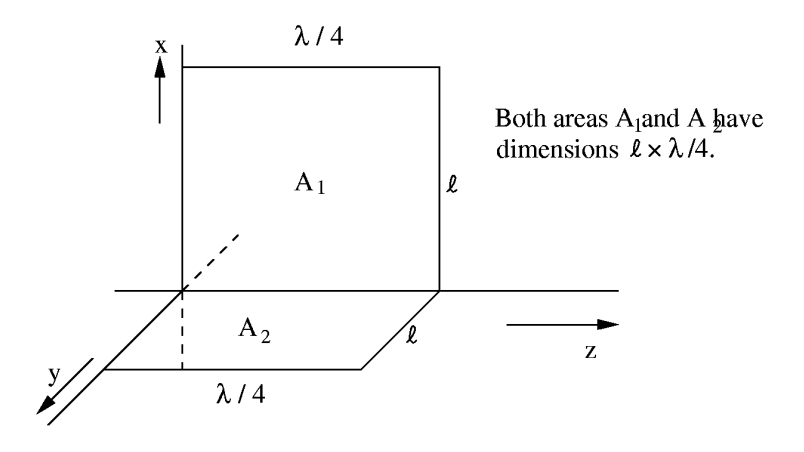
\includegraphics[width=0.7\linewidth]{figs/fig_prob_9.2.png}
    %\caption{Caption}
    %\label{fig:enter-label}
\end{figure}
\\\textbf{Solution}
\\
\\The magnetic flux, $d\Phi_B$, through a small area element of $A_1$ is $B_yl\,dz$. Integrating over the entirety of $A_1$ gives
\[\Phi_B=B_0l\int_{0}^{\lambda/4}\cos(kz-\omega t)\,dz=\frac{B_0l}{k}\left[\sin\left(\frac{2\pi}{\lambda}z-\omega t\right)\right]_{0}^{\lambda/4}=\frac{B_0l}{k}(\cos\omega t+\sin\omega t).\]
Similarly, rate of change of this flux is
\[\frac{d\Phi_B}{dt}=\frac{B_0l}{k}\frac{d}{dt}(\cos\omega t+\sin\omega t)=\frac{B_0l}{\omega/v}\omega(\cos\omega t-\sin\omega t)\]
\begin{equation}
    =B_0lv(\cos\omega t-\sin\omega t).
\end{equation}
Now, for the L.H.S of the Faraday's Law we choose the closed loop enclosing area $A_1$. Moreover, the electric field is perpendicular to the loop at all values of $z$ other than $z=0$ and $z=\lambda/4$. We go around the loop in anticlockwise direction. Thus, the closed loop integral of electric field simplifies to
\[\oint\boldsymbol{\vec{E}}\cdot d\boldsymbol{\vec{l}}=E_0\left(\int_{0}^{l}\cos\left(\frac{2\pi}{\lambda}\times\frac{\lambda}{4}-\omega t\right)\,dl+\int_{l}^{0}\cos\omega t\,dl\right)\]
\begin{equation}
    =E_0l(\sin\omega t-\cos\omega t)
\end{equation}
Substituting equations (1) and (2) into Faraday's Law results in
\[\oint\boldsymbol{\vec{E}}\cdot d\boldsymbol{\vec{l}}=-\frac{d\Phi_B}{dt}\Rightarrow E_0l(\sin\omega t-\cos\omega t)=-B_0lv(\cos\omega t-\sin\omega t)\Rightarrow \frac{E_0}{v}=B_0.\]
In vacuum, the above relation becomes $\frac{E_0}{c}=B_0$. Finally, upon comparing this result with the one obtained via Ampere-Maxwell Law, we obtain
\[\frac{1}{c}=\mu_0\epsilon_0c\Rightarrow c=\frac{1}{\sqrt{\mu_0\epsilon_0}}\]
which is indeed the “speed of light" in vacuum and is approximately equal to $3\times10^8\,$ms$^{-1}$.

\subsubsection*{Problem 9.3 - A standing Electromagnetic Wave}
A wave solution to Maxwell's Equations is given by $\boldsymbol{\vec{E}}=E_0\boldsymbol{\hat{x}}\cos(2\sqrt{3}z)\cos(7\times10^{10}t)$ where $z$ is measured in centimeters and $t$ in seconds.
\begin{enumerate}
    \item[(a)]What is the wavelength and the frequency (in Hz) of the wave?
    \item[(b)]What is the index of refraction, $n$, of the medium?
    \item[(c)]Give the expression for the associated magnetic field, $\boldsymbol{\vec{B}}$, in terms of $E_0$, $z$ and $t$.
    \item[(d)]What is the time averaged Poynting vector for $x=y=3$, $z=\sqrt{3}$?
\end{enumerate}
\textit{Note: Part (c) is not as easy as it may seem. Your solution must satisfy all Maxwell's equations.}
\\
\\\textbf{Solution(a \& b)}
\\
\\Electric field is given in the form of
\[\boldsymbol{\vec{E}}=E_0\boldsymbol{\hat{x}}\cos kz\cos\omega t\]
where $k=\frac{2\pi}{\lambda}$ and $f=\frac{\omega}{2\pi}$. Thus, from these equations, $\lambda=\frac{2\pi}{2\sqrt{3}}=1.8\,$cm and $f=\frac{7\times10^{10}}{2\pi}=1.1\times10^{10}\,$Hz. Similarly the refractive index, $n$, is given by
\[n=\frac{c}{v}=\frac{kc}{\omega}=\frac{2\sqrt{3}\times3\times10^{10}}{7\times10^{10}}\approx1.5.\]
\textbf{Solution(c)}
\\
\\The electric field vector can be written as superposition of two traveling waves, one in the $+z$ and the other in $-z$ direction.
\[\boldsymbol{\vec{E}}=E_0\boldsymbol{\hat{x}}\cos(2\sqrt{3}z)\cos(7\times10^{10}t)=\frac{1}{2}E_0\boldsymbol{\hat{x}}\left(\cos(2\sqrt{3}z-7\times10^{10}t)+\cos(2\sqrt{3}z+7\times10^{10}t)\right)\]
We know that direction of corresponding magnetic field is given by $\boldsymbol{\vec{k}}\times\boldsymbol{\vec{E}}$, thus the magnetic field for wave traveling in $+z$ direction is in $+y$ direction and the other way around (magnetic field can only be along the $y-$axis as propagation of waves and electric fields are along the $z$ and $x-$axis respectively). Therefore,
\[\boldsymbol{\vec{B}}=\frac{1}{2}B_0\boldsymbol{\hat{y}}\left(\cos(2\sqrt{3}z-7\times10^{10}t)-\cos(2\sqrt{3}z+7\times10^{10}t)\right)=B_0\boldsymbol{\hat{y}}\sin(2\sqrt{3}z)\sin(7\times10^{10}t)\]
where $B_0$ is given by $\frac{E_0}{c}$ in vacuum and $\frac{nE_0}{c}$ in any other medium.
\\
\\\textbf{Solution(d)}
\\
\\Poynting vector for the given scenario is
\[\boldsymbol{\vec{S}}=\frac{\boldsymbol{\hat{x}}\times\boldsymbol{\hat{y}}}{\mu_0}\left(E_0\cos(2\sqrt{3}z)\cos(7\times10^{10}t)B_0\sin(2\sqrt{3}z)\sin(7\times10^{10}t)\right).\]
Time average of the function $\sin(\omega t)\cos(\omega t)$ for any value of $\omega$ and $t$ is zero. Hence, there is no transmission of energy ($\boldsymbol{\bar{S}}=0$) in this case for all points in space (including the ones mentioned in problem). 


\subsubsection*{Problem 9.4 - Polarization of Electromagnetic Radiation}
\begin{enumerate}
    \item[(a)]Describe the polarization state of the plane E-M waves represented by the following equations for the electric field $\boldsymbol{\vec{E}}(x,t)$ ($E_x=0$ \textit{in all three cases}):
    \begin{enumerate}
        \item[(1)]$E_y=E_0\sin(kx-\omega t)$, $E_z=4E_0\sin(kx-\omega t)$
        \item[(2)]$E_y=-E_0\cos(kx+\omega t)$, $E_z=E_0\sin(kx+\omega t)$
        \item[(3)]$E_y=2E_0\cos(kx-\omega t+\frac{\pi}{2})$, $E_z=-2E_0\sin(kx-\omega t)$
    \end{enumerate}
    \item[(b)]In each case, give the corresponding equations for the magnetic field, $\boldsymbol{\vec{B}}$. Assume $\omega/k=c$.
\end{enumerate}
\textbf{Solution(a)}
\\
\\At any point in space, the polarization states are linear in (1), circular in (2) and linear in (3). This can be visualized if we plot the electric fields in the $y-z$ plane.
\\
\\\textbf{Solution(b)}
\\
\\As already mentioned in previous problems, direction of corresponding magnetic field is $\boldsymbol{\vec{k}}\times\boldsymbol{\vec{E}}$ and magnitude is $B=\frac{E}{c}$. Thus, the equations for the magnetic fields are
\[\,\,\,(1):\,\boldsymbol{\vec{B}}=\frac{E_0}{c}\left(\sin(kx-\omega t)\boldsymbol{\hat{z}}-4\sin(kx-\omega t)\boldsymbol{\hat{y}}\right)\]
\[(2):\,\boldsymbol{\vec{B}}=\frac{E_0}{c}\left(\cos(kx+\omega t)\boldsymbol{\hat{z}}+\sin(kx+\omega t)\boldsymbol{\hat{y}}\right)\]
\[\,\,\,\,\,\,\,\,\,\,\,\,\,\,\,\,\,\,\,\,(3):\,\boldsymbol{\vec{B}}=\frac{2E_0}{c}\left(\cos(kx-\omega t+\pi/2)\boldsymbol{\hat{z}}+\sin(kx-\omega t)\boldsymbol{\hat{y}}\right)\]

\subsubsection*{Problem 9.5 - Snell's law in action $\Rightarrow$ Dispersion!}
A parallel beam of light containing two wavelengths, $\lambda_1=465\,$nm and $\lambda_2=652\,$nm, enters the silicate flint glass of an equilateral prism (see diagram below). At what angle does each beam leave the prism (give angle with normal to the face)?
\begin{figure}[h]
    \centering
    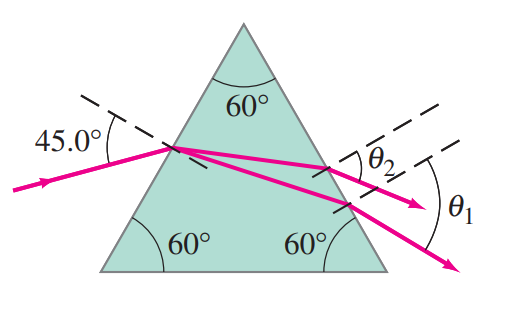
\includegraphics[width=0.4\linewidth]{figs/fig_prob_9.5.png}
   % \caption{Caption}
  %  \label{fig:enter-label}
\end{figure}
\\\textbf{Solution}
\\
\\Refractive index of medium outside the prism ($n_O$) for both wavelengths is 1 and inside the prism ($n_I$) is 1.685 for $\lambda_1$ and 1.625 for $\lambda_2$. The angle of refraction, $\gamma$, inside the prism is given by
\[n_0\sin45=n_I\sin\gamma\Rightarrow\gamma=\sin^{-1}\left(\frac{n_O}{n_I}\sin45\right).\]
The angle, $\phi$, which the refracted ray makes with the other side of the prism is
\[\phi=180-60-(90-\gamma)=30+\sin^{-1}\left(\frac{n_O}{n_I}\sin45\right)\]
and the angle, $\alpha$, that this refracted ray makes with the normal before coming out of the prism is
\[\alpha=90-\phi=60-\sin^{-1}\left(\frac{n_O}{n_I}\sin45\right).\]
Finally, the angle $\theta$, the refracted ray makes with the normal when it comes out of the prism is 
\[n_I\sin\alpha=n_O\sin\theta\Rightarrow\theta=\sin^{-1}\left(\frac{n_I}{n_O}\sin\alpha\right)\]
\[\theta=\sin^{-1}\left(\frac{n_I}{n_O}\sin\left(60-\sin^{-1}\left(\frac{n_O}{n_I}\sin45\right)\right)\right)\]
For $\lambda_1$, $\theta_1\approx76.2$° and for $\lambda_2$, $\theta_2\approx66$°.


\subsubsection*{Problem 9.6 - Snell's law in action $\Rightarrow$ Fiber optics!}
A beam of light enters the end of an optic fiber. Show that we can guarantee total internal reflection at the side surface of the material (at point A), if the index of refraction is greater than about 1.42. In other words, regardless of the angle $\alpha$, the 
light beam reflects back into the material at point A, assuming air outside.
\begin{figure}[h]
    \centering
    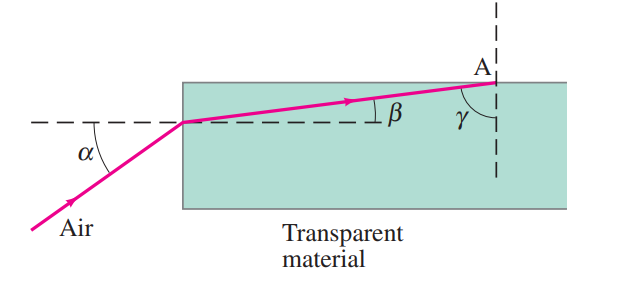
\includegraphics[width=0.55\linewidth]{figs/fig_prob_9.6.png}
  %  \caption{Caption}
 %   \label{fig:enter-label}
\end{figure}
\\\textbf{Solution}
\\
\\Applying Snell's Law at the point of entrance of beam gives
\[\sin\alpha=n\sin\beta.\]
For the worst case scenario, when refraction of light is most improbable, $\alpha\rightarrow90$°. Moreover, $\beta=90-\gamma$. Now the relation becomes
\[n\sin(90-\gamma)=1\Rightarrow n\cos\gamma=1\Rightarrow n^2\cos^2\gamma=1\]
\[n^2\left(1-\sin^2\gamma\right)=1\Rightarrow n^2=1+n^2\sin^2\gamma\Rightarrow\gamma=\sin^{-1}\left(\frac{\sqrt{n^2-1}}{n}\right)\]
When beam emerges from the side of the material, Snell's Law gives the following relation
\[n\sin\gamma=\sin\theta.\]
When total internal reflection is about to occur, $\gamma$ is equal to the critical angle $\theta_c$ and $\theta=90$°. Now we have
\[n\sin\theta_c=1\Rightarrow\theta_c=\sin^{-1}\left(\frac{1}{n}\right).\]
Total internal reflection does not occur when
\[\gamma>\theta_c\Rightarrow\sin^{-1}\left(\frac{\sqrt{n^2-1}}{n}\right)>\sin^{-1}\left(\frac{1}{n}\right)\Rightarrow\sqrt{n^2-1}>1\Rightarrow n>\sqrt{2}\,\,\,\text{or}\,\,\,1.42.\]

\end{document}
